\section{Design REST Api}
\subsection{Introduction}
\begin{flushleft}
Cette section représente le fonctionnement de l'API REST sous forme d'un diagramme de classes. Ce schéma montre les interactions entre l'API, le serveur et les utilisateurs. Les fonctionnalités implémentées dans le diagramme de classe de l'application sont reprises sous forme de requêtes liées à l'API.
\end{flushleft}

\subsection{Gestion d'un utlisateur}
\begin{flushleft}
Lorsqu'un utilisateur interagit avec l'application lors de sa connexion, une requête entrante est envoyée à l'API avec les informations de connexion (un mail, un mot de passe, un nom et un type\footnote{client ou fournisseur}).
\end{flushleft}

\begin{flushleft}
Une fois l'utilisateur créé, une requête sortante est renvoyée à l'application. Ici, 3 possibilités de requêtes sont fournies : 201 - Created, 401 - Unauthorized, 404 - Not Found. Les requêtes 401 et 404 sont erreurs renvoyant un message et le code de l'erreur. Quant à la requête 201, celle-ci met à jour l'application. Cette requête va donc renvoyer un message et le code de la requête. L'application ayant été mis à jour avec les nouvelles données passées en paramètres lors de la requête.
\end{flushleft}

\subsection{Ajout de données}
\begin{flushleft}
Lors d'une interaction avec l'API, il est possible d'ajouter ou de créer des données grâce à une requête "POST". Celle-ci permet notament la création de contrats, de portefeuilles, de propositons de contrats pour les fournisseur et l'ajout d'une méthode de consommation. Si l'interaction est validée, la requête "201 - Created" est renvoyée. Une fois la requête validée, la classe ayant appelée la requête est mis à jour avec les données passées en paramètre.
\end{flushleft}
\newpage
\subsection{Affichage de données}
\begin{flushleft}
Parmi les fonctionnalités disponible pour un utilisateur, la possibilité de voir une liste de certains objets lui appartenant en fait partie. Lors d'une requête "GET", l'API va lister tous les éléments répondant à la requêtes et répondant aux critères mis en paramètres.
\end{flushleft}

\subsection{Modification/Suppression de données}
\begin{flushleft}
Lorsqu'une modification de données est souhaitée, la classe contenant l'objet à modifier effectue une requête "PUT" correspondante. Si la modification est correctement effectuée, l'API renvoie un code "200 - OK" vers une classe "Changed". La suppression de données se base sur le même principe. La classe renvoie une requete "DELETE" supprimant donc l'objet correspondant aux critères et retournant la classe "Changed".
\end{flushleft}

\subsection{Conclusion}
\begin{flushleft}
En conclusion, un utilisateur peut gérer ses données à l'aide de requêtes POST, PUT, GET, DELETE. Ces appels de requêtes sont faites par les classes gestionnaires des objets qu'elles contiennent. Si les critères ne sont pas remplis ou sont invalides, une erreur est renvoyée en fonction du cas.
\newpage

\end{flushleft}
\subsection{Schéma}
\begin{figure}[h]
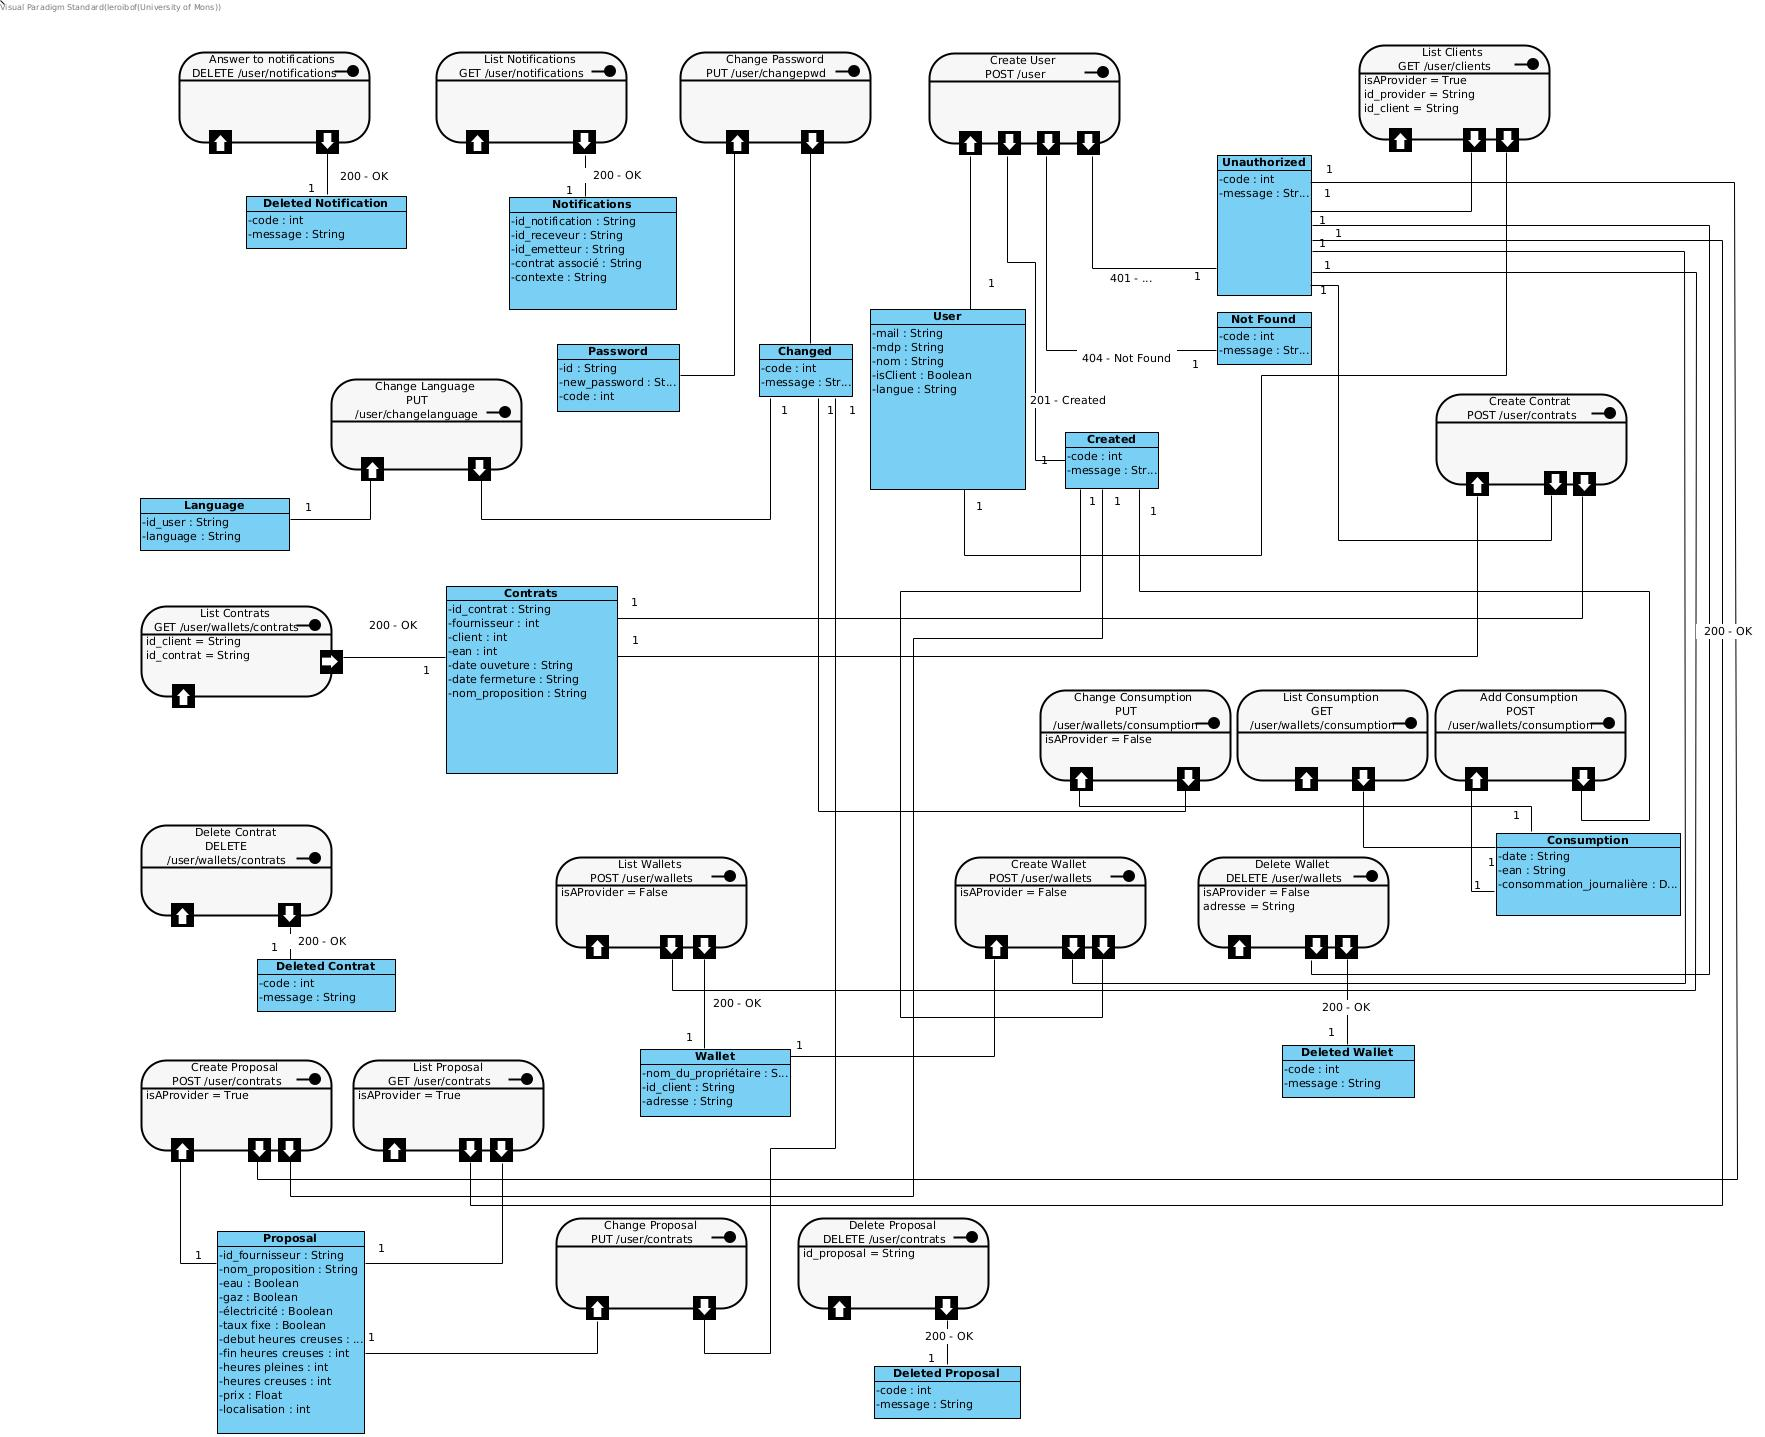
\includegraphics[scale=0.2]{Base/apirest/img/apirest.jpg}
\end{figure}

